\chapter{Related Work}
\label{chap:related_work}
This chapter provides an overview of the existing literature on art tracking with IoT and blockchains, highlighting previous research, methods, and findings related to the research question. Lastly, we also provide an overview of this field's state of the art.

\section{Existing Solutions using IoT and Blockchain}
The combination of these two technologies in industrial systems and supply chains has been a "hot trend" in recent years \cite{industryiot}.

\textcite{modum.io} present a solution to monitor necessary data while transporting medical products. Upon delivery, the collected data is checked for compliance by a smart contract and then stored on the blockchain. There the data is immutable and verifiable by any party.

The proposed system comprises back-end, front-end, and \gls{iot} sensor devices. The architecture and components of the system are shown in Figure \ref{fig:modum.io}.

\begin{figure}[ht]
    \centering
    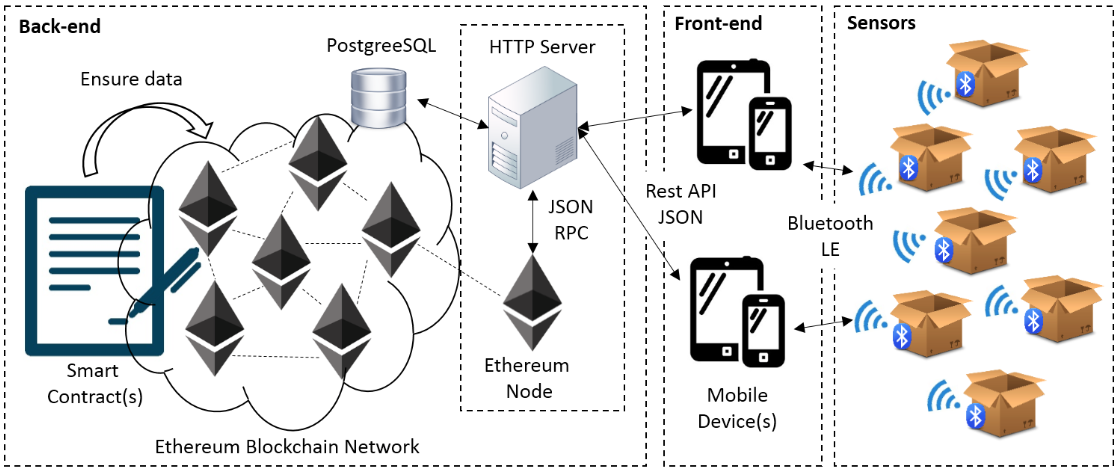
\includegraphics[width=0.8\textwidth]{diagrams/modum_architecutre.png}
    \caption{Modum.io AG Blockchain Architecture \cite{modum.io}}
    \label{fig:modum.io}
\end{figure}

In addition to the Ethereum Blockchain Network, modum.io uses a relational database to store raw temperature data and user credentials. The mobile clients download the temperature data via Bluetooth from the sensors and submit it to the server, which sends it to the \gls{sc} to evaluate the regulatory compliance and store the result \gls{on-chain}.

\textcite{everledger}, is a digital transparency company providing technology solutions to increase transparency in global supply chains. They use blockchain to track and verify the authenticity of high-value assets such as diamonds, wine, and art. Their platform allows users to track the entire lifecycle of an asset, from production to ownership, using a secure and transparent blockchain-based ledger. Everledger mainly focuses on fraud detection, verification, and provenance records by issuing digital certificates stored on a private blockchain.

\textcite{authena}, is a Swiss-based company that provides a platform for tracking and verifying the authenticity of physical assets using blockchain technology and \gls{iot}. Their platform offers three main products:
\begin{itemize}
    \item AUTHENA SHIELD: A tamper-proof end-to-end authenticity solution.
    \item AUTHENA L1VE: Real-time tracking of location and environmental conditions across countries and distribution channels.
    \item AUTHENA M3TA: Creating a secure link between physical product and its twin in the Metaverse.
\end{itemize}

\section{Existing Art Tracking Solutions using IoT and Blockchain}
Blockchain technology has been proposed as a promising solution to the challenges faced in the creative industry, such as issues related to the monetization of intellectual property and the provenance and authenticity of creative work. \cite{creativeindustry} Especially technologies like smart contracts and \glspl{nft} have shown the potential of blockchain technology to revolutionize the art market by enabling greater transparency, accountability, and traceability.  

\textcite{nftopportunities} has shown the benefits of \glspl{nft} protecting digital assets by proving their existence and ownership. \textcite{creativeindustry} has suggested the application of \glspl{nft} beyond digital art, proposing to physically tag an \gls{iot} device to an artwork or sculpture to transfer and track ownership. The \gls{iot} device is designed such that an attempt to tamper with the device will result in a blockchain record. This would potentially reduce intermediaries by providing a verifiable certificate that proves ownership, custodial-history, and authenticity of a physical asset.

\textcite{artchain}, for example, developed a blockchain-based trading system for artworks that uses \glspl{nft} to represent physical artworks. Introducing traceability, irreversibility, and transparency into the art market. 

In this regard, \textcite{nftminter} has proposed an advanced \gls{nft} Minter for a blockchain-based artwork trading system. 

\textcite{artrentalblockchain} developed an artwork rental system based on blockchain technology to facilitate lending artwork collections.
% TODO: where to add this? Another related study by \textcite{zkdet} proposes a traceable and privacy-preserving data exchange scheme based on \gls{nft} and \gls{zkp}

\textcite{artory}, is a company employing these concepts to tokenize physical artworks to create a secure record of art pieces' provenance and ownership. 

The related work thus far has mainly shown the benefits of representing physical goods as digital \glspl{nft} on the blockchain. There is little work to be found on using IoT devices to monitor environmental parameters while transporting artworks. However, a study by \textcite{pactart} developed an \gls{iot} architecture called PACT-ART that employs advanced computing techniques like data mining and business process intelligence to predict a future state of the process and point out any possible violation from it. This system does not incorporate blockchain technology.
